\documentclass[aspectratio=169]{beamer}

\usetheme[progressbar=frametitle]{metropolis}
%\usepackage{italian, babel}
\setbeamertemplate{frame numbering}[none]
\useoutertheme{metropolis}
\useinnertheme{metropolis}
\usefonttheme{serif}
\usepackage{graphics}
%\usecolortheme{spruce}
\setbeamercolor{background canvas}{bg=white}

\title[Titolo in basso a destra]{Lezione di Matematica: Derivate}
\subtitle{sottotitolo lezione}
\date{\today}
\author{Diego Fantinelli}
\institute{Matematica per il Liceo}

\begin{document}

\begin{frame}
  \maketitle
\end{frame}

\begin{frame}{Indice}
  \tableofcontents
\end{frame}

\section{Introduzione alla Parabola}

\begin{frame}{Definizione}
La parabola è una curva piana che ha la proprietà di essere simmetrica rispetto a un asse chiamato "asse di simmetria" e di avere la forma di un arco di circonferenza.
  
 \begin{figure}[htbp]
  \centering
    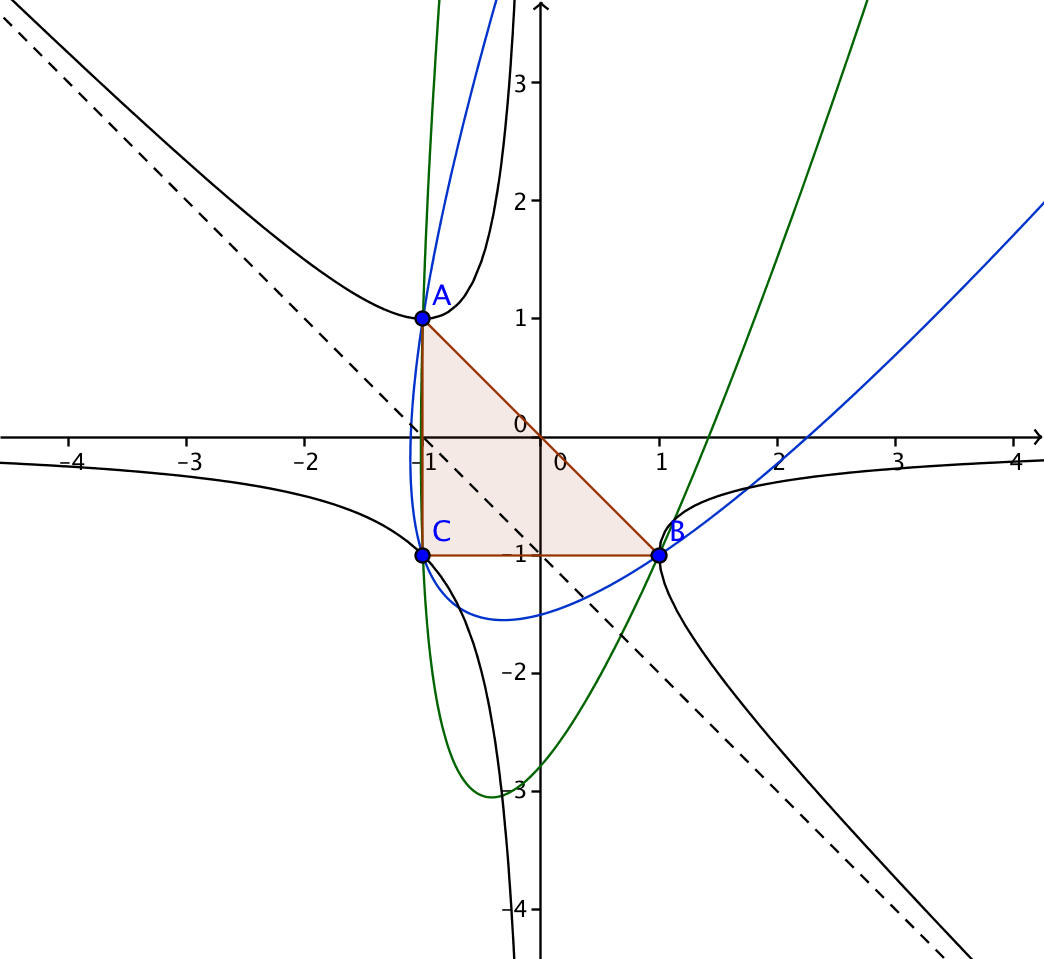
\includegraphics[width=0.35\textwidth]{parabola.png}
      \caption{Esempio grafico di una parabola.}
      \label{fig:parabola}
 \end{figure}  
\end{frame}

\section{Equazione della Parabola}

\begin{frame}{Equazione standard della Parabola}
  L'equazione standard della parabola è:
  
  $$y = ax^2 + bx + c$$
  
  dove $a$, $b$ e $c$ sono costanti reali.
  
  Se $a > 0$, la parabola si apre verso l'alto, mentre se $a < 0$, la parabola si apre verso il basso.
  
  Se $b = c = 0$, l'asse di simmetria della parabola è l'asse $y$.
\end{frame}

\section{Proprietà della Parabola}

\begin{frame}{Focale e Direttrice}
  La parabola ha due punti speciali: il fuoco e la direttrice.
\end{frame}

\section{Proprietà della Iperbole}

\begin{frame}{Focale e Direttrice}
  La parabola ha due punti speciali: il fuoco e la direttrice.
\end{frame}

\end{document}
